% talk a little about initial page table conditions:
%     paging not on, but virtual mostly mapped direct to physical,
%     which is what things look like when we turn paging on as well
%     since paging is turned on after we create first process.
%   mention why still have SEG_UCODE/SEG_UDATA?
%   do we ever really say what the low two bits of %cs do?
%     in particular their interaction with PTE_U
%   sidebar about why it is extern char[]
\chapter{Page tables}
\label{CH:MEM}

Page tables are the most popular mechanism through which the operating
system provides each process with its own private address space and
memory.  Page tables determine what memory addresses mean, and what
parts of physical memory can be accessed. They allow xv6 to isolate
different process's address spaces and to multiplex them onto a single
physical memory. Page tables are a popular design because they provide
a level of indirection that allow operating systems to perform many
tricks. Xv6 performs a few tricks: mapping the same memory
(a trampoline page) in several address spaces, and guarding kernel and
user stacks with an unmapped page. The rest of this chapter explains
the page tables that the RISC-V hardware provides and how xv6 uses
them.

%% 
\section{Paging hardware}
%% 
As a reminder,
RISC-V instructions (both user and kernel) manipulate virtual addresses.
The machine's RAM, or physical memory, is indexed with physical
addresses.
The RISC-V page table hardware connects these two kinds of addresses,
by mapping each virtual address to a physical address.

\begin{figure}[t]
\center
\includegraphics[scale=0.5]{fig/riscv_address.pdf}
\caption{RISC-V virtual and physical addresses, with a simplified
logical page table.}
\label{fig:riscv_address}
\end{figure}

Xv6 runs on Sv39 RISC-V, which means that only the bottom 39
bits of a 64-bit virtual address are used; the top 25 bits
are not used.
In this Sv39 configuration, a
RISC-V page table is logically an array of $2^{27}$ (134,217,728)
\indextext{page table entries (PTEs)}.  Each PTE contains a 44-bit
physical page number (PPN) and some flags. The paging hardware
translates a virtual address by using the top 27 bits of the 39 bits
to index into the page table to find a PTE, and making a 56-bit
physical address whose top 44 bits come from the PPN in the PTE
and whose bottom 12 bits are copied from the original virtual address.
Figure~\ref{fig:riscv_address} shows this
process with a logical view of the page table as a simple array of PTEs
(see Figure~\ref{fig:riscv_pagetable} for a fuller story).
A page table
gives the operating system control over virtual-to-physical address
translations at the granularity of aligned chunks of 4096 ($2^{12}$)
bytes.  Such a chunk is called a \indextext{page}.

\begin{figure}[t]
\center
\includegraphics[scale=0.5]{fig/riscv_pagetable.pdf}
\caption{RISC-V address translation details.}
\label{fig:riscv_pagetable}
\end{figure}

In Sv39 RISC-V, the top 25 bits of a virtual address are not used for
translation. The physical address also has room for growth: there is
room in the PTE format for the physical page number to grow by another
10 bits.  The designers of RISC-V chose these numbers based on
technology predictions.  $2^{39}$ bytes is 512 GB, which should be
enough address space for applications running on RISC-V
computers. $2^{56}$ is enough physical memory space for the near
future to fit many I/O devices and RAM chips. If
more is needed, the RISC-V designers have defined Sv48 with 48-bit
virtual addresses~\cite{riscv:priv}.

As 
Figure~\ref{fig:riscv_pagetable} shows,
a RISC-V CPU translates a virtual address into a physical in
three steps.  A page table is stored
in physical memory as a three-level tree.
The root of the tree is a
4096-byte page-table page that contains 512 PTEs, which contain the physical
addresses for page-table pages in the next level of the tree.  Each of those
pages contains 512 PTEs for the final level in the tree.  The paging
hardware uses the top 9 bits of the 27 bits to select a PTE in the
root page-table page, the middle 9 bits to select a PTE in a page-table page in the
next level of the
tree, and the bottom 9 bits to select the final PTE.
(In Sv48 RISC-V a page table has four levels, and bits 39 through 47
of a virtual address index into the top-level.)

If any of the three PTEs required to translate an address
is not present, the paging hardware raises a \indextext{page-fault exception}, leaving it up
to the kernel to handle the exception (see Chapter~\ref{CH:TRAP}).

The three-level structure of Figure~\ref{fig:riscv_pagetable} allows a
memory-efficient way of recording PTEs, compared to the single-level
design of Figure~\ref{fig:riscv_address}.  In the common case in which
large ranges of virtual addresses have no mappings, the three-level
structure can omit entire page directories.  For example, if an
application uses only a few pages starting at address zero, then the
entries 1 through 511 of the top-level page directory are invalid, and
the kernel doesn't have to allocate pages those for 511 intermediate
page directories.  Furthermore, the kernel also doesn't have to
allocate pages for the bottom-level page directories for those 511
intermediate page directories. So, in this example, the three-level
design saves 511 pages for intermediate page directories and
$511\times512$ pages for bottom-level page directories.

Although a CPU walks the three-level structure in hardware as part of
executing a load or store instruction, a potential downside of three
levels is that the CPU must load three PTEs from memory to perform the
translation of the virtual address in the load/store instruction to a
physical address.  To avoid the cost of loading PTEs from physical
memory, a RISC-V CPU caches page table entries in a
\indextext{Translation Look-aside Buffer (TLB)}.

Each PTE contains flag bits that tell the paging hardware
how the associated virtual address is allowed to be used.
\indexcode{PTE_V}
indicates whether the PTE is present: if it is
not set, a reference to the page causes an exception (i.e., is not allowed).
\indexcode{PTE_R}
controls whether instructions are allowed to 
read to the page.
\indexcode{PTE_W}
controls whether instructions are allowed to 
write to the page.
\indexcode{PTE_X}
controls whether the CPU may interpret the content
of the page as instructions and execute them.
\indexcode{PTE_U}
controls whether instructions in user mode are allowed
to access the page;
if \indexcode{PTE_U} is not set, the PTE can be used only in supervisor mode.
Figure~\ref{fig:riscv_pagetable}
shows how it all works.
The flags and all other page hardware-related structures are defined in
\fileref{kernel/riscv.h}

To tell a CPU to use a page table, the kernel must
write the physical address of the root page-table page into the 
\texttt{satp}\index{satp@\lstinline{satp}} register.
A CPU will translate all addresses generated by subsequent instructions
using the page table pointed to by its own \texttt{satp}.
Each CPU has its own \texttt{satp} so that different CPUs can run
different processes, each with a private address space described by
its own page table.

From the kernel's point of view, a page table is data stored in
memory, and the kernel creates and modifies page tables using code
much like you might see for any tree-shaped data structure.

A few notes about terms used in this book. \textit{Physical memory}
refers to storage cells in RAM. A byte of physical memory has an
address, called a \textit{physical address}. Instructions that
dereference addresses (such as loads, stores, jumps, and function calls)
use only
virtual addresses, which the paging hardware translates to physical
addresses, and then sends to the RAM hardware to read or write
storage. An \textit{address space} is the set of virtual addresses
that are valid in a given page table; each xv6 process has a separate
user address space, and the xv6 kernel has its own address space as
well. \textit{User memory} refers to a process's user address space
plus the physical memory that the page table allows the process to
access. \textit{Virtual memory} refers to the ideas and techniques
associated with managing page tables and using them to achieve goals
such as isolation.

\begin{figure}[h]
\centering
 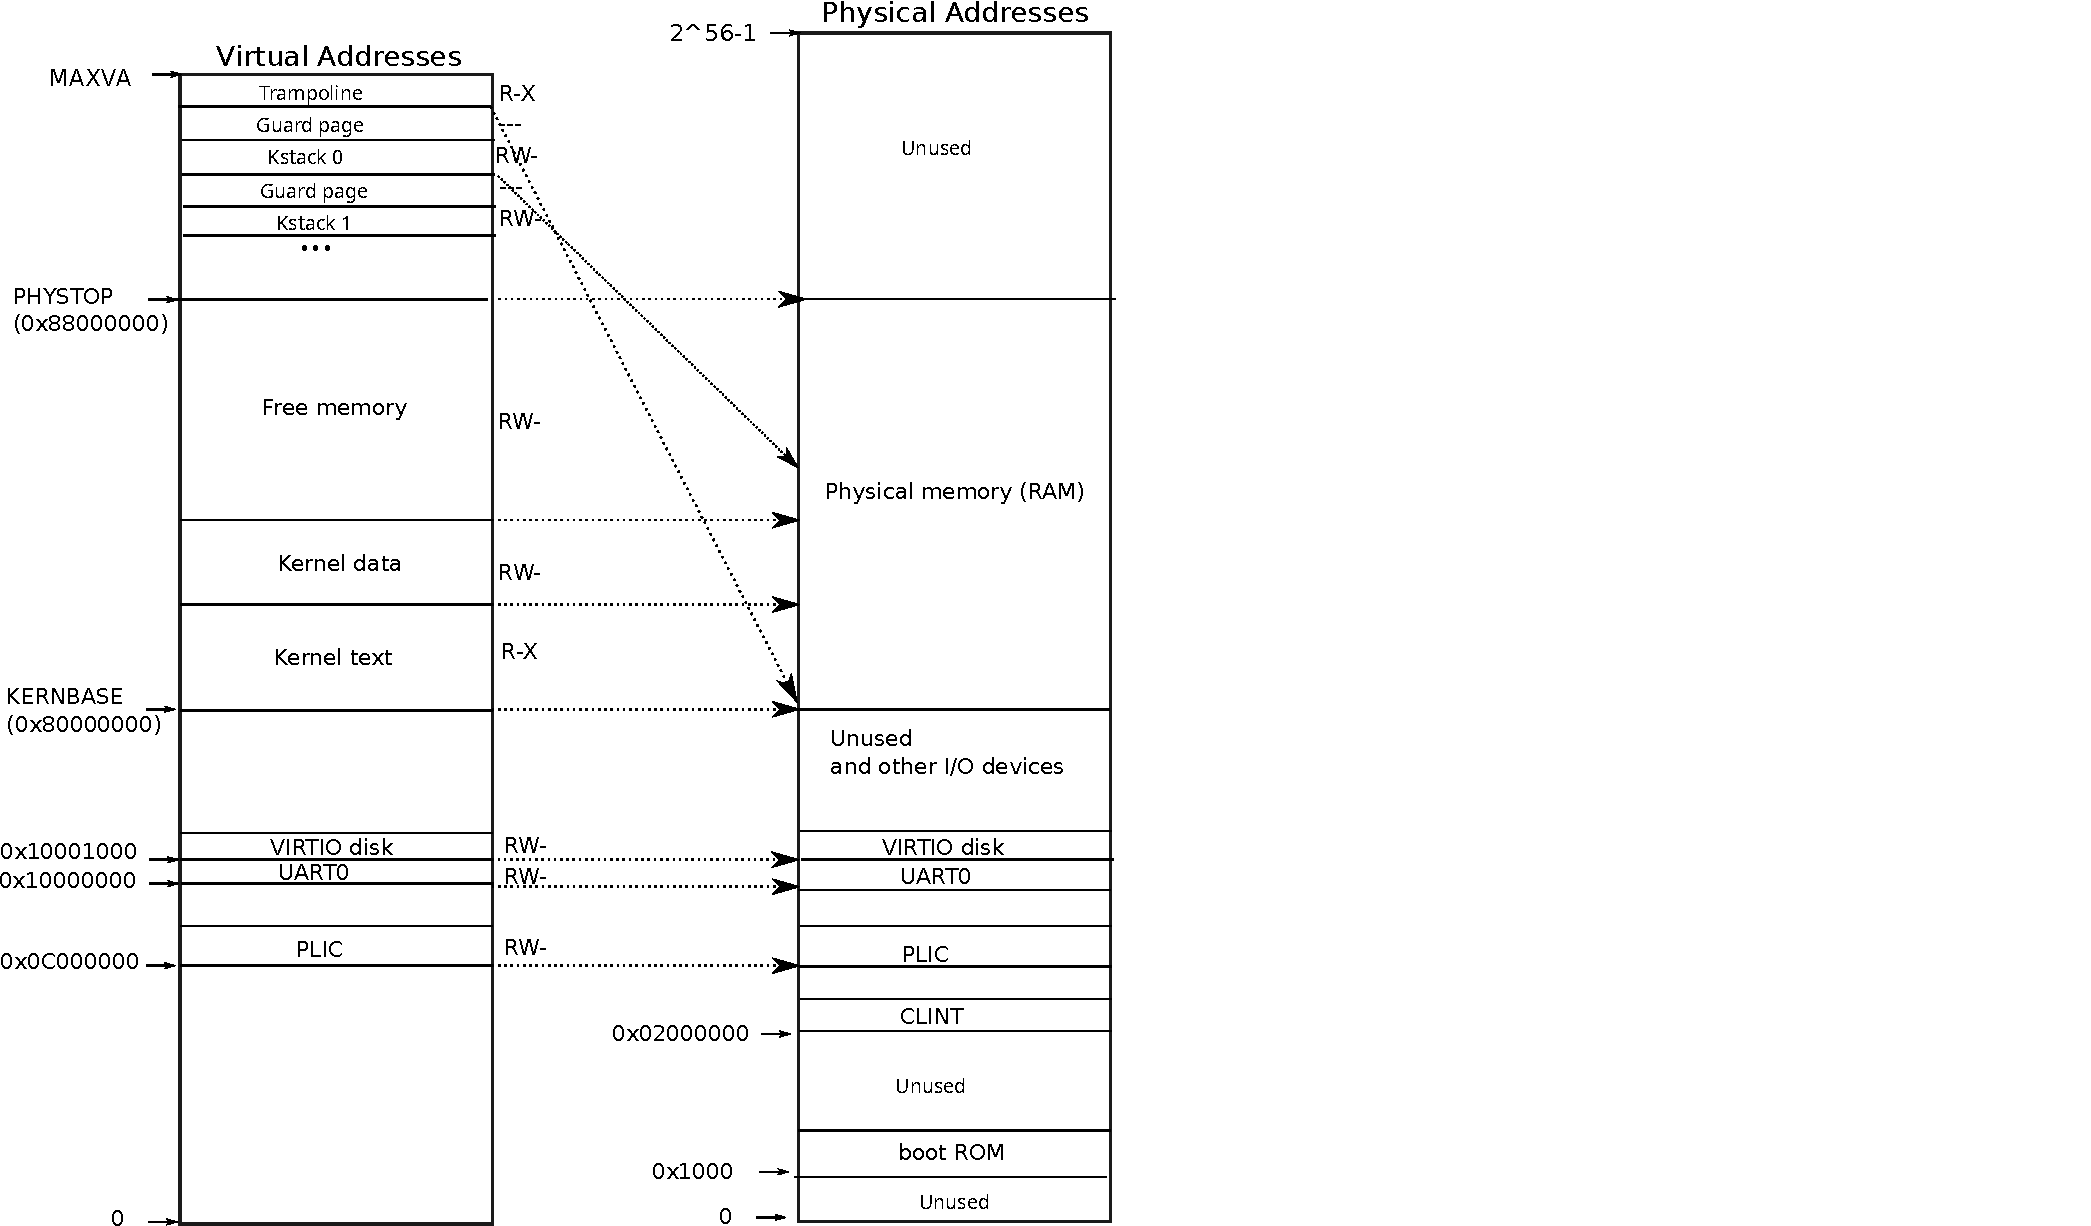
\includegraphics[scale=0.65]{fig/xv6_layout.pdf}
\caption{On the left, xv6's kernel address space.
{\sf \small{RWX}}
refer to PTE read, write, and execute permissions.
On the right, the RISC-V physical address space that
xv6 expects to see.}
\label{fig:xv6_layout}
\end{figure}

%% 
\section{Kernel address space}
%% 
Xv6 maintains one page table per process, describing each
process's user address space, plus a single page table
that describes the kernel's address space.
The kernel configures the layout of its address space to
give itself
access to physical memory and
various hardware resources at predictable virtual addresses.
Figure~\ref{fig:xv6_layout}
shows how this layout maps
kernel virtual addresses to physical addresses.  The file
\fileref{kernel/memlayout.h}
declares the constants for xv6's kernel memory layout.

QEMU simulates a computer that includes RAM (physical memory) starting
at physical address \texttt{0x80000000} and continuing through
at least \texttt{0x88000000}, which xv6 calls \texttt{PHYSTOP}.
The QEMU simulation also
includes I/O devices
such as a disk interface.
QEMU exposes the device interfaces to software as
\indextext{memory-mapped}
control registers that sit below
\texttt{0x80000000}
in the physical address space.
The kernel can interact with the devices by reading/writing
these special physical addresses; such reads and writes communicate
with the device hardware rather than with RAM.
Chapter~\ref{CH:TRAP} explains
how xv6 interacts with devices.

The kernel gets at RAM and memory-mapped device registers
using ``direct mapping;'' that is, mapping the resources at
virtual addresses that are equal to the physical address.
For
example, the kernel itself is located at \lstinline{KERNBASE=0x80000000} in both
the virtual address space and in physical memory.
Direct mapping simplifies kernel code that reads or writes
physical memory. For example, when \lstinline{fork}
allocates user memory for the child process,
the allocator returns the physical address of that memory;
\lstinline{fork} uses that address directly as a virtual
address when it is copying the parent's user memory to the child.

There are a couple of kernel virtual
addresses that aren't direct-mapped:

\begin{itemize}
  
\item The trampoline page. It is mapped at the top of the virtual
  address space; user page tables have this same mapping.
  Chapter~\ref{CH:TRAP} discusses the role of the trampoline
  page, but we see here an interesting use case of page tables; a
  physical page (holding the trampoline code) is mapped twice in the
  virtual address space of the kernel: once at top of the virtual
  address space and once with a direct mapping.

\item The kernel stack pages.  Each process has its own kernel stack,
  which is mapped high so that below it xv6 can leave an unmapped \indextext{guard
    page}.  The guard page's PTE is invalid (i.e.,
  \lstinline{PTE_V} is not set), so that if the kernel overflows
  a kernel stack, it will likely cause an exception and the kernel will panic.
  Without a guard page an overflowing stack would overwrite other kernel memory,
  resulting in incorrect operation. A panic crash is preferable.

\end{itemize}

While the kernel uses its stacks via the high-memory mappings, they
are also accessible to the kernel through a direct-mapped address. An
alternate design might have just the direct mapping, and use the
stacks at the direct-mapped address. In that arrangement, however,
providing guard pages would involve unmapping virtual addresses that
would otherwise refer to physical memory, which would then be hard to
use.

The kernel maps the pages for the trampoline and the kernel text with
the permissions
\lstinline{PTE_R}
and
\lstinline{PTE_X}.
The kernel reads and executes instructions from these pages.
The kernel maps the other pages with the permissions
\lstinline{PTE_R}
and
\lstinline{PTE_W},
so that it can read and write the memory in those pages.
The mappings for the guard pages are invalid.


%% 
\section{Code: creating an address space}
%% 

Most of the xv6 code for manipulating address spaces and
page tables resides in {\tt vm.c}
\lineref{kernel/vm.c:1}.
The central data structure is {\tt pagetable\_t}, which
is really a pointer to a RISC-V root page-table page;
a {\tt pagetable\_t} may be either the kernel
page table, or one of the per-process page tables.
The central functions are {\tt walk},
which finds the PTE for a virtual address,
and {\tt mappages}, which installs PTEs for new mappings.
Functions starting with {\tt kvm} manipulate
the kernel page table; functions starting with {\tt uvm}
manipulate a user page table; other functions are
used for both.
{\tt copyout} and {\tt copyin} copy data to and from
user virtual addresses provided as system call arguments;
they are in {\tt vm.c} because they need to explicitly
translate those addresses in order to find the corresponding
physical memory.

Early in the boot sequence,
\indexcode{main}
calls
\indexcode{kvminit}
\lineref{kernel/vm.c:/^kvminit/}
to create the kernel's page table using
\indexcode{kvmmake}
\lineref{kernel/vm.c:/^kvmmake/}.
This call occurs before xv6 has enabled paging on the RISC-V,
so addresses refer directly to physical memory.
\lstinline{kvmmake}
first allocates a page of physical memory to hold the root page-table page.
Then it calls
\indexcode{kvmmap}
to install the translations that the kernel needs.
The translations include the kernel's
instructions and data, physical memory up to
\indexcode{PHYSTOP},
and memory ranges which are actually devices.
\indexcode{proc_mapstacks}
\lineref{kernel/proc.c:/^proc_mapstacks/}
allocates a kernel stack for each
process. It calls \lstinline{kvmmap} to map each stack at the virtual address generated by
\lstinline{KSTACK}, which leaves room for the invalid stack-guard
pages.

\indexcode{kvmmap} 
\lineref{kernel/vm.c:/^kvmmap/}
calls
\indexcode{mappages}
\lineref{kernel/vm.c:/^mappages/},
which
installs mappings into a page table
for a range of virtual addresses to
a corresponding range of physical addresses.
It does this separately for each virtual address in the range,
at page intervals.
For each virtual address to be mapped,
\lstinline{mappages}
calls
\indexcode{walk}
to find the address of the PTE for that address.
It then initializes the PTE to hold the relevant physical page
number, the desired permissions 
(\lstinline{PTE_W},
\lstinline{PTE_X},
and/or
\lstinline{PTE_R}),
and
\lstinline{PTE_V}
to mark the PTE as valid
\lineref{kernel/vm.c:/perm...PTE_V/}.

\indexcode{walk}
\lineref{kernel/vm.c:/^walk/}
mimics the RISC-V paging hardware as it
looks up the PTE for a virtual address (see
Figure~\ref{fig:riscv_pagetable}).
\lstinline{walk}
descends the page table one level at a time,
using each level's 9 bits of virtual address to
index into the relevant page directory page.
At each level it finds either the PTE of the
next level's page directory page, or the PTE of
final page
\lineref{kernel/vm.c:/pte.=..pagetable/}.
If a PTE in a first or second level page directory
page isn't valid, then the required directory page
hasn't yet been allocated;
if the
\lstinline{alloc}
argument is set,
\lstinline{walk}
allocates a new page-table page and puts its physical address in the PTE.
It returns the address of the PTE in the lowest layer in the tree
\lineref{kernel/vm.c:/return..pagetable/}.

The above code depends on physical memory being direct-mapped into the
kernel virtual address space. For example, as \lstinline{walk} descends levels
of the page table, it pulls the (physical) address of the
next-level-down page table from a PTE \lineref{kernel/vm.c:/pagetable.=..pa.*E2P/},
and then uses that address as a
virtual address to fetch the PTE at the next level down
\lineref{kernel/vm.c:/t..pte.=..paget/}.

\indexcode{main}
calls
\indexcode{kvminithart}
\lineref{kernel/vm.c:/^kvminithart/}
to install the kernel page table.
It writes the physical address of the root page-table page
into the register
\texttt{satp}.
After this the CPU will translate addresses using the kernel
page table.  Since the kernel uses a direct mapping, the now
virtual address of the next instruction will map to the right physical
memory address.

Each RISC-V CPU caches page table entries in a
\indextext{Translation Look-aside Buffer (TLB)}, and when xv6 changes
a page table, it must tell the CPU to invalidate corresponding
cached TLB entries.  If it didn't,
then at some point later the TLB might
use an old cached mapping, pointing to a physical page that in the meantime
has been allocated to another process, and as a result, a process
might be able to scribble on some other process's memory.  The RISC-V
has an instruction \indexcode{sfence.vma} that flushes
the current CPU's TLB.
Xv6 executes {\tt sfence.vma} in {\tt kvminithart}  after reloading the 
\texttt{satp} register, and in the trampoline code that
switches to a user page table before returning to user space
\lineref{kernel/trampoline.S:/sfence.vma/}.

It is also necessary to issue \texttt{sfence.vma} before changing
\texttt{satp}, in order to wait for completion of all outstanding loads and
stores. This wait ensures that preceding updates to the page table have
completed, and ensures that preceding loads and stores use the old
page table, not the new one.

To avoid flushing the complete TLB, RISC-V CPUs may support address
space identifiers (ASIDs)~\cite{riscv:priv}.  The kernel can then
flush just the TLB entries for a particular address space. Xv6
does not use this feature.

\section{Physical memory allocation}

The kernel must allocate and free physical memory at run-time for
page tables,
user memory,
kernel stacks,
and pipe buffers.

Xv6 uses the physical memory between the end of the kernel and
\indexcode{PHYSTOP}
for run-time allocation. It allocates and frees whole 4096-byte pages
at a time. It keeps track of which pages are free by threading a
linked list through the pages themselves. Allocation consists of
removing a page from the linked list; freeing consists of adding the
freed page to the list.
%% 
\section{Code: Physical memory allocator}
%% 

The allocator resides in {\tt kalloc.c} \lineref{kernel/kalloc.c:1}.
The allocator's data structure is a
\textit{free list}
of physical memory pages that are available
for allocation.
Each free page's list element is a
\indexcode{struct run}
\lineref{kernel/kalloc.c:/^struct.run/}.
Where does the allocator get the memory
to hold that data structure?
It store each free page's
\lstinline{run}
structure in the free page itself,
since there's nothing else stored there.
The free list is
protected by a spin lock
\linerefs{kernel/kalloc.c:/^struct.{/,/}/}.
The list and the lock are wrapped in a struct
to make clear that the lock protects the fields
in the struct.
For now, ignore the lock and the calls to
\lstinline{acquire}
and
\lstinline{release};
Chapter~\ref{CH:LOCK} will examine
locking in detail.

The function
\indexcode{main}
calls
\indexcode{kinit}
to initialize the allocator
\lineref{kernel/kalloc.c:/^kinit/}.
\lstinline{kinit}
initializes the free list to hold
every page between the end of the kernel and {\tt PHYSTOP}.
Xv6 ought to determine how much physical
memory is available by parsing configuration information 
provided by the hardware.
Instead xv6 assumes that the machine has
128 megabytes of RAM.
\lstinline{kinit}
calls
\indexcode{freerange}
to add memory to the free list via per-page calls to
\indexcode{kfree}.
A PTE can only refer to a physical address that is aligned
on a 4096-byte boundary (is a multiple of 4096), so
\lstinline{freerange}
uses
\indexcode{PGROUNDUP}
to ensure that it frees only aligned physical addresses.
The allocator starts with no memory;
these calls to
\lstinline{kfree}
give it some to manage.

The allocator sometimes treats addresses as integers
in order to perform arithmetic on them (e.g.,
traversing all pages in
\lstinline{freerange}),
and sometimes uses addresses as pointers to read and
write memory (e.g., manipulating the
\lstinline{run}
structure stored in each page);
this dual use of addresses is the main reason that the
allocator code is full of C type casts.
\index{type cast}

The function
\lstinline{kfree}
\lineref{kernel/kalloc.c:/^kfree/}
begins by setting every byte in the
memory being freed to the value 1.
This will cause code that uses memory after freeing it
(uses ``dangling references'')
to read garbage instead of the old valid contents;
hopefully that will cause such code to break faster.
Then
\lstinline{kfree}
prepends the page to the free list:
it casts
\lstinline{pa}
to a pointer to
\lstinline{struct}
\lstinline{run},
records the old start of the free list in
\lstinline{r->next},
and sets the free list equal to
\lstinline{r}.
\indexcode{kalloc}
removes and returns the first element in the free list.

\section{Process address space}

Each process has its own page table, and when xv6 switches between
processes, it also changes page tables.
Figure~\ref{fig:processlayout} shows a process's address space in more
detail than Figure~\ref{fig:as}.  A process's user memory starts at
virtual address zero and can grow up to \texttt{MAXVA}
\lineref{kernel/riscv.h:/MAXVA/}, allowing a process to address in
principle 256 Gigabytes of memory.

A process's address space consists of pages that contain the text of
the program (which xv6 maps with the permissions \lstinline{PTE_R},
\lstinline{PTE_X}, and \lstinline{PTE_U}), pages that contain the
pre-initialized data of the program, a page for the stack, and pages
for the heap.  Xv6 maps the data, stack, and heap with the permissions
\lstinline{PTE_R}, \lstinline{PTE_W}, and \lstinline{PTE_U}.

Using permissions within a user address space is a common technique to
harden a user process.  If the text were mapped with
\lstinline{PTE_W}, then a process could accidentally modify its own
program; for example, a programming error may cause the program to
write to a null pointer, modifying instructions at address 0, and then
continue running, perhaps creating more havoc.  To detect such errors
immediately, xv6 maps the text without \lstinline{PTE_W}; if a program
accidentally attempts to store to address 0, the hardware will refuse
to execute the store and raises a page fault (see
Section~\ref{sec:pagefaults}).  The kernel then kills the process and
prints out an informative message so that the developer can track down
the problem.

Similarly, by mapping data without \lstinline{PTE_X}, a user program
cannot accidentally jump to an address in the program's data and start
executing at that address.

In the real world, hardening a process by setting permissions
carefully also aids in defending against security attacks.  An
adversary may feed carefully-constructed input to a program (e.g., a
Web server) that triggers a bug in the program in the hope of turning
that bug into an exploit~\cite{aleph:smashing}.  Setting permissions
carefully and other techniques, such as randomizing of the layout of the
user address space, make such attacks harder.

The stack is a single page, and is shown with the initial contents as
created by exec.  Strings containing the command-line arguments, as
well as an array of pointers to them, are at the very top of the
stack.  Just under that are values that allow a program to start at
\lstinline{main} as if the function \lstinline{main(argc},
\lstinline{argv)} had just been called.

To detect a user stack overflowing the allocated stack memory, xv6
places an inaccessible guard page right below the stack by clearing
the \lstinline{PTE_U} flag. If the user stack overflows and the
process tries to use an address below the stack, the hardware will
generate a page-fault exception because the guard page is inaccessible
to a program running in user mode. A real-world operating system might
instead automatically allocate more memory for the user stack when it
overflows.

When a process asks xv6 for more user memory, xv6 grows the process's
heap. Xv6 first uses {\tt kalloc} to allocate physical pages.
It then adds PTEs to the process's page table that point
to the new physical pages.
Xv6 sets the
\lstinline{PTE_W},
\lstinline{PTE_R},
\lstinline{PTE_U},
and
\lstinline{PTE_V}
flags in these PTEs.
Most processes do not use the entire user address space;
xv6 leaves
\lstinline{PTE_V}
clear in unused PTEs.

We see here a few nice examples of use of page tables.  First,
different processes' page tables translate user addresses to different
pages of physical memory, so that each process has private user
memory.  Second, each process sees its memory as having contiguous
virtual addresses starting at zero, while the process's physical
memory can be non-contiguous.  Third, the kernel maps a page with
trampoline code at the top of the user address space (without
\lstinline{PTE_U}), thus a single page of physical memory shows up in
all address spaces, but can be used only by the kernel.

\begin{figure}[t]
\center
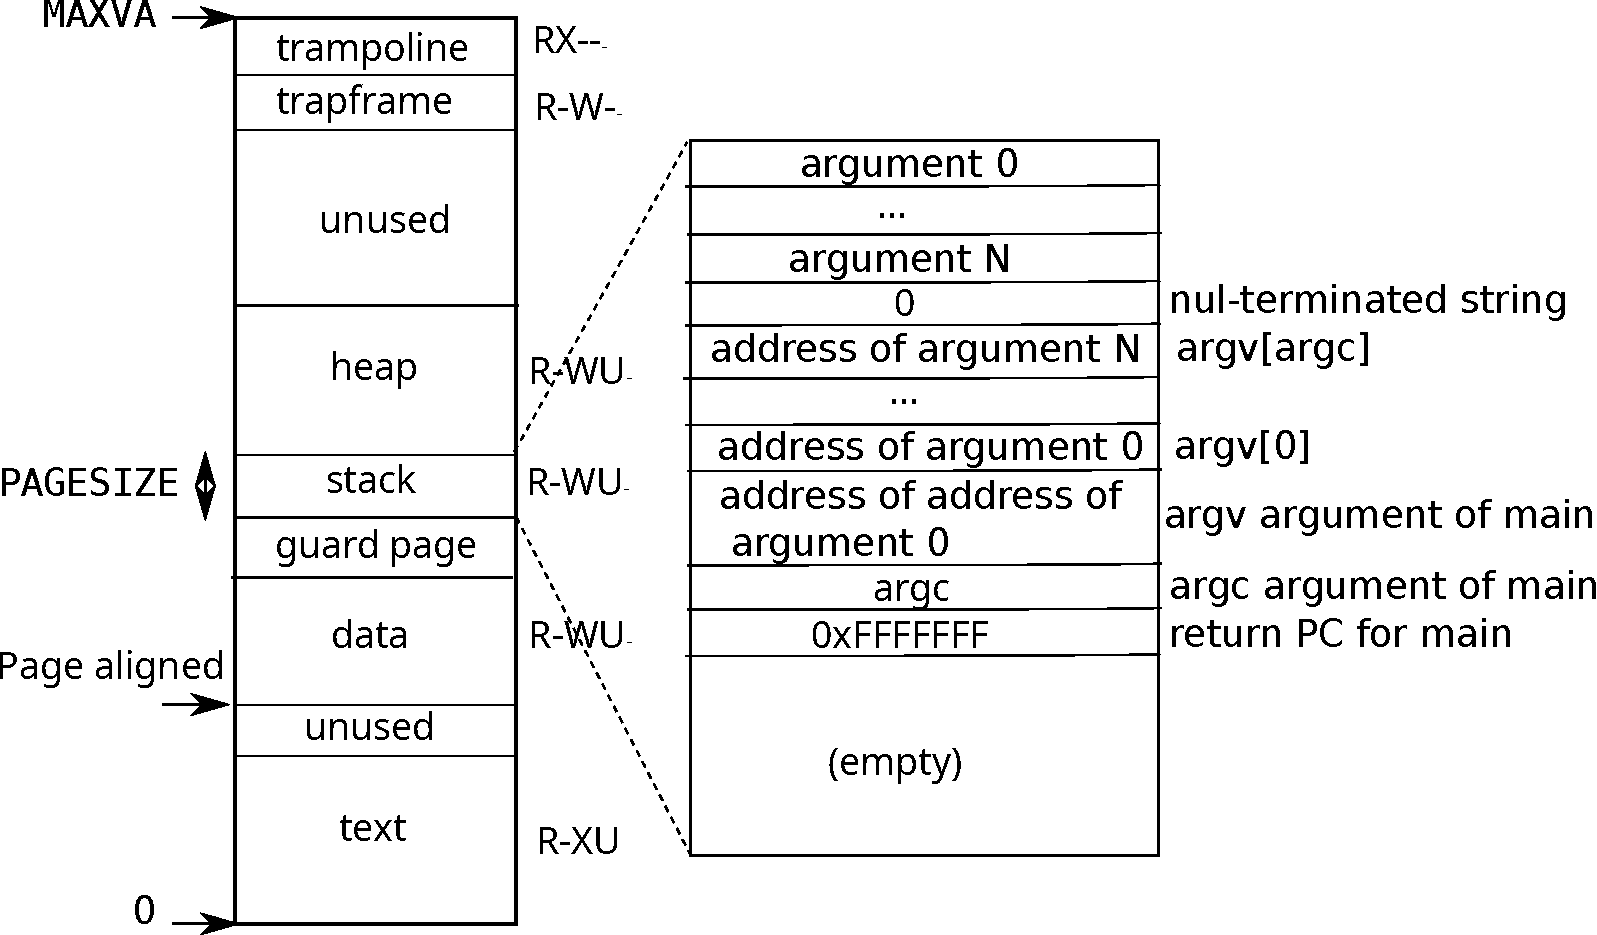
\includegraphics[scale=0.5]{fig/processlayout.pdf}
\caption{A process's user address space, with its initial stack.}
\label{fig:processlayout}
\end{figure}

\section{Code: sbrk}

\lstinline{sbrk}
is the system call for a process to shrink or grow its memory. The system
call is implemented by the function
\lstinline{growproc}
\lineref{kernel/proc.c:/^growproc/}.
\lstinline{growproc} calls \lstinline{uvmalloc} or
\lstinline{uvmdealloc}, depending on whether \lstinline{n} is positive
or negative.
\lstinline{uvmalloc}
\lineref{kernel/vm.c:/^uvmalloc/}
allocates physical memory with {\tt kalloc},
and adds PTEs to the user page table with {\tt mappages}.
\lstinline{uvmdealloc} calls
{\tt uvmunmap}
\lineref{kernel/vm.c:/^uvmunmap/},
which uses {\tt walk} to find PTEs and
{\tt kfree} to free the physical memory they refer to.

Xv6 uses a process's page table not just to tell the hardware how to
map user virtual addresses, but also as the only record of which
physical memory pages are allocated to that process. That is the
reason why freeing user memory (in {\tt uvmunmap}) requires
examination of the user page table.

%% 
\section{Code: exec}
%% 
\lstinline{exec} is a system call that replaces a process's
user address space with data read from a file, called a binary
or executable file.
A binary is typically the output of the compiler and linker,
and holds machine instructions and program data.
\lstinline{exec} \lineref{kernel/exec.c:/^exec/} opens the
named binary \lstinline{path} using \indexcode{namei}
\lineref{kernel/exec.c:/namei/}, which is explained in
Chapter~\ref{CH:FS}.  Then, it reads the ELF header. Xv6 binaries
are formatted in the widely-used \indextext{ELF format}, defined in
\fileref{kernel/elf.h}.  An ELF binary consists of an ELF header,
\indexcode{struct elfhdr} \lineref{kernel/elf.h:/^struct.elfhdr/},
followed by a sequence of program section headers,
\lstinline{struct proghdr} \lineref{kernel/elf.h:/^struct.proghdr/}.  Each
\lstinline{progvhdr} describes a section of the application that must
be loaded into memory; xv6 programs have two program section
headers: one for instructions and one for data.

The first step is a quick check that the file probably contains an
ELF binary.
An ELF binary starts with the four-byte ``magic number''
\lstinline{0x7F},
\lstinline{`E'},
\lstinline{`L'},
\lstinline{`F'},
or
\indexcode{ELF_MAGIC}
\lineref{kernel/elf.h:/ELF_MAGIC/}.
If the ELF header has the right magic number,
\lstinline{exec}
assumes that the binary is well-formed.

\lstinline{exec}
allocates a new page table with no user mappings with
\indexcode{proc_pagetable}
\lineref{kernel/exec.c:/proc_pagetable/},
allocates memory for each ELF segment with
\indexcode{uvmalloc}
\lineref{kernel/exec.c:/uvmalloc/},
and loads each segment into memory with
\indexcode{loadseg}
\lineref{kernel/exec.c:/loadseg/}.
\lstinline{loadseg}
uses
\indexcode{walkaddr}
to find the physical address of the allocated memory at which to write
each page of the ELF segment, and
\indexcode{readi}
to read from the file.

The program section header for
\indexcode{/init},
the first user program created with
\lstinline{exec},
looks like this:
\begin{footnotesize}
\begin{verbatim}
# objdump -p user/_init

user/_init:     file format elf64-little

Program Header:
0x70000003 off    0x0000000000006bb0 vaddr 0x0000000000000000
                                       paddr 0x0000000000000000 align 2**0
         filesz 0x000000000000004a memsz 0x0000000000000000 flags r--
    LOAD off    0x0000000000001000 vaddr 0x0000000000000000
                                       paddr 0x0000000000000000 align 2**12
         filesz 0x0000000000001000 memsz 0x0000000000001000 flags r-x
    LOAD off    0x0000000000002000 vaddr 0x0000000000001000
                                       paddr 0x0000000000001000 align 2**12
         filesz 0x0000000000000010 memsz 0x0000000000000030 flags rw-
   STACK off    0x0000000000000000 vaddr 0x0000000000000000
                                       paddr 0x0000000000000000 align 2**4
         filesz 0x0000000000000000 memsz 0x0000000000000000 flags rw-
\end{verbatim}
\end{footnotesize}

We see that the text segment should be loaded at virtual address 0x0
in memory (without write permissions) from content at offset
0x1000 in the file. We also see that the data should be loaded at
address 0x1000, which is at a page boundary, and without executable
permissions.

A program section header's
\lstinline{filesz}
may be less than the
\lstinline{memsz},
indicating that the gap between them should be filled
with zeroes (for C global variables) rather than read from the file.
For
\lstinline{/init}, the data
\lstinline{filesz}
is 0x10 bytes and
\lstinline{memsz}
is 0x30 bytes,
and thus
\indexcode{uvmalloc}
allocates enough physical memory to hold 0x30 bytes, but reads only 0x10 bytes
from the file
\lstinline{/init}.

Now
\indexcode{exec}
allocates and initializes the user stack.
It allocates just one stack page.
\lstinline{exec}
copies the argument strings to the top of the stack
one at a time, recording the pointers to them in
\indexcode{ustack}.
It places a null pointer at the end of what will be the
\indexcode{argv}
list passed to
\lstinline{main}.
The first three entries in
\lstinline{ustack}
are the fake return program counter,
\indexcode{argc},
and
\lstinline{argv}
pointer.

\lstinline{exec}
places an inaccessible page just below the stack page,
so that programs that try to use more than one page will fault.
This inaccessible page also allows
\lstinline{exec}
to deal with arguments that are too large;
in that situation,
the
\indexcode{copyout}
\lineref{kernel/vm.c:/^copyout/}
function that
\lstinline{exec}
uses to copy arguments to the stack will notice that
the destination page is not accessible, and will
return -1.

During the preparation of the new memory image,
if
\lstinline{exec}
detects an error like an invalid program segment,
it jumps to the label
\lstinline{bad},
frees the new image,
and returns -1.
\lstinline{exec}
must wait to free the old image until it
is sure that the system call will succeed:
if the old image is gone,
the system call cannot return -1 to it.
The only error cases in
\lstinline{exec}
happen during the creation of the image.
Once the image is complete,
\lstinline{exec}
can commit to the new page table
\lineref{kernel/exec.c:/pagetable.=.pagetable/}
and free the old one
\lineref{kernel/exec.c:/proc_freepagetable/}.

\lstinline{exec}
loads bytes from the ELF file into memory at addresses specified by the ELF file.
Users or processes can place whatever addresses they want into an ELF file.
Thus
\lstinline{exec}
is risky, because the addresses in the ELF file may refer to the kernel, accidentally
or on purpose. The consequences for an unwary kernel could range from
a crash to a malicious subversion of the kernel's isolation mechanisms
(i.e., a security exploit).
Xv6 performs a number of checks to avoid these risks.
For example
\lstinline{if(ph.vaddr + ph.memsz < ph.vaddr)}
checks for whether the sum overflows a 64-bit integer.
The danger is that a user could construct an ELF binary with a
\lstinline{ph.vaddr}
that points to a user-chosen address,
and
\lstinline{ph.memsz}
large enough that the sum overflows to 0x1000, which will look like a
valid value. In an older version of xv6 in which the user address
space also contained the kernel (but not readable/writable in user
mode), the user could choose an address that corresponded to kernel
memory and would thus copy data from the ELF binary into the kernel.
In the RISC-V version of xv6 this cannot happen, because the kernel has
its own separate page table;
\lstinline{loadseg}
loads into the process's page table, not in the kernel's page table.

It is easy for a kernel developer to omit a crucial check, and
real-world kernels have a long history of missing checks whose absence
can be exploited by user programs to obtain kernel privileges.  It is likely that xv6 doesn't do a complete job of validating
user-level data supplied to the kernel, which a malicious user program might be able to exploit to circumvent xv6's isolation.
%% 
\section{Real world}
%% 

Like most operating systems, xv6 uses the paging hardware for memory
protection and mapping.  Most operating systems make far more
sophisticated use of paging than xv6 by combining paging and
page-fault exceptions, which we will discuss in
Chapter~\ref{CH:TRAP}.

Xv6 is simplified by the kernel's use of a direct map between virtual
and physical addresses, and by its assumption that there is physical
RAM at address 0x80000000, where the kernel expects to be loaded. This
works with QEMU, but on real hardware it turns out to be a bad idea;
real hardware places RAM and devices at unpredictable physical
addresses, so that (for example) there might be no RAM at 0x80000000,
where xv6 expect to be able to store the kernel. More serious kernel
designs exploit the page table to turn arbitrary hardware physical
memory layouts into predictable kernel virtual address layouts.

RISC-V supports protection at the level of physical addresses,
but xv6 doesn't use that feature.

On machines with lots of memory
it might make sense to use
RISC-V's support for ``super pages.''
Small pages make sense
when physical memory is small, to allow allocation and page-out to disk
with fine granularity.
For example, if a program
uses only 8 kilobytes of memory, giving it a whole 4-megabyte super-page
of physical memory is wasteful.
Larger pages make sense on machines with lots of RAM,
and may reduce overhead for page-table manipulation.

The xv6 kernel's lack of a {\tt malloc}-like allocator that can
provide memory for small objects prevents the kernel from using
sophisticated data structures that would require dynamic allocation.
A more elaborate kernel
would likely allocate many different sizes of small blocks,
rather than (as in xv6) just 4096-byte blocks;
a real kernel
allocator would need to handle small allocations as well as large
ones.

Memory allocation is a perennial hot topic, the basic problems being
efficient use of limited memory and
preparing for unknown future requests~\cite{knuth}.  Today people care more about speed than
space efficiency.
%% 
\section{Exercises}
%% 

\begin{enumerate}
  
\item Parse RISC-V's device tree to find the amount of physical memory
the computer has.

\item Write a user program that grows its address space by one byte by calling
\lstinline{sbrk(1)}.
Run the  program and investigate the page table for the program before the call
to
\lstinline{sbrk}
and after the call to
\lstinline{sbrk}.
How much space has the kernel allocated?  What does the
PTE
for the new memory contain?

\item Modify xv6 to use super pages for the kernel.

\item Unix implementations of
\lstinline{exec}
traditionally include special handling for shell scripts.
If the file to execute begins with the text
\lstinline{#!},
then the first line is taken to be a program
to run to interpret the file.
For example, if
\lstinline{exec}
is called to run
\lstinline{myprog}
\lstinline{arg1}
and
\lstinline{myprog} 's
first line is
\lstinline{#!/interp},
then
\lstinline{exec}
runs
\lstinline{/interp}
with command line
\lstinline{/interp}
\lstinline{myprog}
\lstinline{arg1}.
Implement support for this convention in xv6.

\item Implement address space layout randomization for the kernel.

\end{enumerate}
